\documentclass[12pt, a4paper]{report}
\usepackage[english]{babel}
\usepackage{newlfont}
\usepackage{xcolor}
\usepackage[urlbordercolor=blue]{hyperref}
\usepackage{mathtools}
\usepackage{amssymb}
\usepackage{csquotes}
\usepackage[toc,page]{appendix}
\usepackage[labelfont=bf]{caption}

\usepackage{tikz}
\usepackage[compat=1.1.0]{tikz-feynman}
\usetikzlibrary{patterns}

\graphicspath{ {./images} }

\usepackage[
    backend=biber,
    style=phys,
    articletitle=true,
    biblabel=brackets,
    chaptertitle=true,
    eprint=true,
    maxbibnames=8
]{biblatex}
\addbibresource{bibliography.bib}

\textwidth=450pt\oddsidemargin=0pt

% Enable arXiv linking
\DeclareFieldFormat{eprint:arxiv}{%
  \mkbibbrackets{\href{https://arxiv.org/abs/#1}{\nolinkurl{#1}}}%
}

% Italics title
\DeclareFieldFormat
  [article,inproceedings,incollection,unpublished]
  {title}{\mkbibemph{#1}}

% Italics title and enable link-title keyword
\DeclareFieldFormat{title}{%
  \ifkeyword{link-title}
    {\iffieldundef{url}
      {\mkbibemph{#1}}
      {\mkbibemph{\href{\thefield{url}}{#1}}}}
    {\mkbibemph{#1}}}

\DeclareFieldFormat[article,inbook,incollection,inproceedings,patent,thesis,unpublished]{title}{%
  \ifkeyword{link-title}
    {\iffieldundef{url}
      {\mkbibemph{#1\isdot}}
      {\mkbibemph{\href{\thefield{url}}{#1}\isdot}}}
    {\mkbibemph{#1\isdot}}}

\begin{document}


\begin{titlepage}
\begin{center}
{{\Large{\textsc{Alma Mater Studiorum $\cdot$ Universit\`a di Bologna}}}} 
\rule[0.1cm]{15.8cm}{0.1mm}
\rule[0.5cm]{15.8cm}{0.6mm}
\\\vspace{3mm}

{\small{\bf Dipartimento di Fisica e Astronomia “Augusto Righi”\\
Corso di Laurea in Fisica}}

\end{center}

\vspace{23mm}

\begin{center}
{\LARGE{\bf Sommerfeld enhancement of Dark Matter signals at telescopes}}\\
\end{center}

\vspace{50mm} \par \noindent

\begin{minipage}[t]{0.47\textwidth}
{\large{\bf Relatore: \vspace{2mm}\\
Dott. Filippo Sala}}
\end{minipage}
%
\hfill
%
\begin{minipage}[t]{0.47\textwidth}\raggedleft
{\large{\bf Presentata da:
\vspace{2mm}\\
Luca Zoppetti}}
\end{minipage}

\vspace{40mm}

\begin{center}
Anno Accademico 2024/2025
\end{center}

\end{titlepage}



\newpage
\
\thispagestyle{empty}
\newpage

\begin{abstract}
  La materia oscura è stata accettata negli ultimi decenni come possibile soluzione a diverse incongruenze fra previsioni e misure a livello cosmologico, alcune delle quali vengono brevemente presentate nell'introduzione di questo lavoro. Un grande filone di esperimenti di rivelazione indiretta sta attualmente cercando prove della sua esistenza osservando tramite telescopi i raggi cosmici provenienti da molteplici fonti astronomiche. Sebbene questo non abbia ancora portato a una scoperta confermata di segnali di materia oscura, ha permesso di porre limiti molto stringenti sulla cross section della sua annichilazione. Il confronto di questi limiti con la cross section prevista teoricamente per la materia oscura nel caso in cui essa sia una ``reliquia termica'' composta da WIMPs permette di porre limiti anche sulla massa della particella stessa. L'obiettivo della tesi è studiare come l'effetto quantistico non-relativistico detto \emph{Sommerfeld enhancement} possa impattare di diversi ordini di grandezza questi limiti. Con riferimento ai dati provenienti dalla collaborazione Fermi-LAT, si mostra che in assenza di \emph{Sommerfeld enhancement} il limite inferiore sulla massa è di circa \(80 \mathrm{GeV} \), mentre in presenza di \emph{Sommerfeld enhancement} diventa circa \(9.9 \mathrm{TeV} \). L'intero studio è condotto nell'approssimazione di Coulomb, per cui l'interazione è mediata da un mediatore non massivo. La validità di questa approssimazione viene verificata alla fine del lavoro.
\end{abstract}

\newpage
\
\thispagestyle{empty}
\newpage

\tableofcontents

\newpage
\
\thispagestyle{empty}
\newpage

\chapter{Introduction}\label{chap:introduction}

\section{Structure of the thesis}
The objective of this work is to review the quantum-mechanical effect known as Sommerfeld enhancement \cite{Sommerfeld_1931}, and understand how its presence can deeply affect the theoretical predictions of some relevant dark matter models. This will be done by considering the theoretical framework laid out by Arkani-Hamed et al. in \cite{Arkani_2009} and by applying it to the experimental limits on the dark matter annihilation cross-section found by Profumo et al. \cite{Profumo_2018} through direct observation of gamma-ray production from dwarf spheroidal galaxies orbiting the Milky Way. The thesis is structured in three parts:
\begin{itemize}
	\item In Chapter \ref{chap:introduction}, I introduce the concept of dark matter and of its indirect detection. At the end of the chapter, a detailed description of Sommerfeld enhancement and its use in this work will be given.
	\item In Chapter \ref{chap:derivation}, I will thoroughly explain the mathematical derivation that leads to the final expression of the Sommerfeld enhancement factor in the so-called Coulomb approximation.
	\item In Chapter \ref{chap:implications}, I will apply the concepts and formulae set out in the first two chapters to derive lower bounds on the dark matter mass with and without Sommerfeld enhancement. After this, I will check whether the Coulomb approximation was a good approximation in this case, and I will draw the conclusions of this research.
\end{itemize}

The whole thesis uses natural units where \(c=\hbar=G=1\). Numerical calculations had to be performed to compute the enhanced cross-section. For completeness, the code I wrote is open-source on \href{https://github.com/LuckeeDev/bachelor-thesis}{GitHub}.

\section{Dark matter}

\section{Indirect detection}

\section{Sommerfeld enhancement}

Initially studied by Sommerfeld in 1931 \cite{Sommerfeld_1931}, the Sommerfeld enhancement is an effect arising in non-relativistic quantum mechanics where the introduction of a long-range potential affects the cross-section of a process happening locally at the origin.

One can easily picture the effect by making an analogy with classical mechanics. Consider an object traveling with velocity \(v\) towards a star of radius \(R\) and mass \(M\): if we neglect gravity, the cross-section for falling into the star is simply the area occupied by the star \(\sigma _0=\pi R^2\). However, if we consider gravity, the cross-section increases because the object can be dragged from further away into the star. This means that the cross-section is actually \(\sigma = \pi b_{max}^2 \), where \(b_{max}\) is the largest the impact parameter can be for the distance of closest approach of the orbit to be \(R\) \cite{Arkani_2009, Cirelli_2024}. We can determine the enhancement factor by imposing conservation of energy and angular momentum, and get
\begin{equation}
	\sigma = \sigma _0 \left( 1+ \frac{v_{esc} ^2}{v ^2} \right), 
\end{equation}
where \(v_{esc} ^2 = 2M / R\) is the escape velocity from the surface of the star. The cross-section can thus be greatly enhanced at velocities \(v \ll v_{esc} \).

In quantum mechanics, something similar can happen with the introduction of a long-range potential. Consider, for instance, an annihilation happening locally at the origin thanks to a Hamiltonian of the type \(H_{ann} = U_{ann} \delta (\vec{r})\). The rate of the process will be proportional to the squared modulus of the wavefunction at the origin \(\vert \psi ^{(0)}(0) \vert^2 \). If we introduce a potential, the original wavefunction will get distorted and will have a different value at the origin, now making the rate proportional to \(\vert \psi (0) \vert^2 \). The Sommerfeld enhancement factor is defined as the ratio between the two cross-sections, and therefore between the squared moduli of the wavefunctions:
\begin{equation}\label{eq:sommerfeld_def}
	S = \frac{\sigma }{\sigma _0} = \frac{\vert \psi (0) \vert ^2}{\vert \psi ^{(0)}(0) \vert ^2}
\end{equation}

Although dark matter does not interact electromagnetically and gravity is irrelevant at these scales, Sommerfeld enhancement can be extremely relevant for dark matter theory in the hypothesis that the dark matter particles couple to an attractive force carrier with Compton wavelength longer than \((\alpha M_{DM})^{-1} \), where \(\alpha\) is the strength of the interaction and \(M_{DM} \) is the mass of the dark matter particle. In other words, we're referring to a light force carrier \(\phi \) with mass \(m_{\phi } \lesssim \alpha M_{DM} \). This light force carrier could be the mediator of a yet unknown ``dark interaction'': this claim exists in several theories of physics beyond the standard model \cite{Arkani_2009}.

Since the mediator is expected to be massive, the most natural way to model the long-range interaction would be a classic Yukawa potential:
\begin{equation}
	V(r) = -\frac{\alpha }{r} e^{-m_{\phi } r}
\end{equation}
However, in the limit of a massless mediator, the potential tends to a simple Coulomb potential and the associated Schrödinger equation admits an analytic solution. Intuitively, one can make the approximation of a massless mediator, and thus an infinite-range force, when the range of the force is larger than the De Broglie wavelength of the system \((\mu v_{rel})^{-1} \), where \(\mu \) is the reduced mass and \(v_{rel} \) is the relative velocity of the two particles \cite{Sala_2019}. This translates into the following constraint for two particles with identical mass \(M_{DM} \):
\begin{equation}
	\frac{M_{DM} v_{rel} }{2m_{\phi } }\geq 1
\end{equation}
If the Coulomb approximation is not valid, one should instead use the Yukawa potential and solve the equation numerically, or else approximate it with the Hulthen potential to be able to solve the problem analytically:
\begin{equation}\label{eq:Coulomb_approx}
	V_H(r) = \frac{\alpha \kappa m_{\phi } e^{-\kappa m_{\phi }r }}{1- e^{-\kappa m_{\phi }r }},
\end{equation}
where the approximation is most accurate for \(\kappa \thickapprox 1.74\) \cite{Cirelli_2024}. In the following, I will always assume a massless mediator, and I will later check if it was indeed a good approximation.

One more reason for being interested in Sommerfeld enhancement is that, as we will see in the following, it is velocity-dependent, and therefore allows for different cross-sections at freeze-out and today. In particular, it allows higher cross-sections today compared to the one that is required to give the correct dark matter thermal relic abundance (\(\langle \sigma v \rangle_{relic}=4.4\times 10^{-26} \mathrm{cm^3 s^{-1}}\) for non-self-conjugate dark matter).

\chapter{Solving the equation}

\section{Reduction to one-dimensional problem}

The two-body problem involving the supposed new mediator \(\phi \) and the two identical Dark Matter particles can be expressed through the following non-relativistic Schrödinger equation:
\begin{equation}
	-\frac{1}{2m} \nabla_1 ^2 \Psi(\vec{r}_1,\vec{r}_2)  - \frac{1}{2m} \nabla_2 ^2 \Psi(\vec{r}_1,\vec{r}_2)  + V(\vert \vec{r}_1 - \vec{r}_2 \vert ) \Psi(\vec{r}_1,\vec{r}_2) =E \Psi (\vec{r}_1,\vec{r}_2),
\end{equation}
where \(m\) is the mass of the two identical Dark Matter particles, \(\Psi\) is the wavefunction of the system, \(V\) is the potential describing the interaction mediated by \(\phi \) and \(E\) is the total energy of the system. The first step to solving this equation is to rewrite it as a one-body problem in the centre-of-mass frame through the following substitutions: \(\vec{r} \coloneqq  \vec{r}_1 - \vec{r}_2\), which represents the distance between the two particles, and \(\vec{R} \coloneqq (\vec{r}_1 + \vec{r}_2) / 2\), which is the position of the centre-of-mass. Since the two particles have the same mass, the reduced mass \(\mu \) is just \(\mu = m / 2\). One can easily show that the following relations hold:
\begin{equation}
	\nabla _1 = \frac{1}{2} \nabla _R + \nabla _r
	\qquad
	\nabla _2 = \frac{1}{2} \nabla _R - \nabla _r
\end{equation}
To do this, I will call \(x^i_1, x^i_2, X^i \) and \(x^i\) the coordinates of \(\vec{r}_1, \vec{r}_2, \vec{R} \) and \(\vec{r}\) respectively. By applying the chain rule,
\begin{equation}
	\frac{\partial }{\partial x^i_1} = \frac{\partial X^i}{\partial x^i_1} \frac{\partial }{\partial X^i} + \frac{\partial x^i}{\partial x^i_1} \frac{\partial }{\partial x^i} = \frac{1}{2} \frac{\partial }{\partial X^i} + \frac{\partial }{\partial x^i},
\end{equation}
and a similar result can be obtained for the second particle. With this result, the equation turns into a simpler form:
\begin{equation}
	\left[- \frac{1}{8\mu} \nabla _R^{2} - \frac{1}{2\mu } \nabla _r^2 + V(r)\right] \Psi (\vec{R},\vec{r})= E \Psi (\vec{R},\vec{r})
\end{equation}
This equation clearly suggests that the wavefunction can be separated into the product of a function describing the centre of mass and another one describing the system as seen from the centre-of-mass frame: \(\Psi (\vec{R},\vec{r}) = \psi_R \psi _r\). The problem can therefore be studied as two separate problems, and for the sake of this derivation we will only focus on the centre-of-mass description of it. The centre-of-mass Schrödinger equation is
\begin{equation}
	\left[- \frac{1}{2\mu }\nabla _r^2 + V(r)\right]\psi _r = E_{CM} \psi _r
\end{equation}
Energy is conserved, so we can write \(E_{CM} \) as the energy when the two particles are infinitely far apart, or else as the sum of their kinetic energies when the potential is substantially negligible. In the centre-of-mass frame, the two particles have the same speed \(v\) but opposite direction of movement, resulting in a relative velocity \(v_{rel} = 2v\). This means that \(E_{CM} = mv^2 = \frac{1}{2} \mu v_{rel}^2\), which is the energy of a particle of mass \(\mu \) moving at a speed of \(v_{rel} \). One can make the standard substitution \(k=\mu v_{rel} \) and obtain
\begin{equation}
	\left[- \frac{1}{2\mu } \nabla ^2 + V(r)\right] \psi _k (\vec{r}) = \frac{k^2}{2\mu } \psi _k (\vec{r}),
\end{equation}
which is the standard description of a particle moving in a potential. To simplify the notation, I decide to drop the subscript r on the \(\nabla _r ^2\) operator. In the following, I might omit to specify the dependence of the potential and of the wavefunction on the position.

\section{Reduction to radial problem}

If there was no potential, a valid solution would be a simple plane wave traveling in the \(z\) direction:
\begin{equation}
	\psi _k^{(0)} = e^{ikz} 
\end{equation}
If we add a spherically symmetric interaction centred at the origin, initially modeled as a typical Yukawa potential \(V(r) =- \frac{\alpha}{r} e^{-m_{\phi } r }\), we expect the wavefunction to behave as the sum of a plane wave (the incident wave that gets scattered by the potential) and a spherical wave with intensity dependent on the angle formed with the \(z\) axis (the scattered wave) as \(r\) goes to infinity:
\begin{equation}\label{deriv:asymptotic}
	\psi _k \to e^{ikz} + f(\theta ) \frac{e^{ikr} }{r} \text{ as } r\to \infty 
\end{equation}
We know from standard quantum mechanics that solutions to the Schrödinger equation with a spherically symmetric potential can be separated as
\begin{equation}
	\psi_{klm} (r,\theta,\varphi) = R_{kl} (r) Y_l^m(\theta , \varphi ),
\end{equation}
where the radial functions \(R_{kl} \) satisfy the radial equation
\begin{equation}\label{deriv:radial}
	-\frac{1}{2\mu } \frac{1}{r^2} \frac{\mathrm{d}}{\mathrm{d}r}\left(r^2 \frac{\mathrm{d}}{\mathrm{d}r}  R_{kl}\right) + \left(V(r)+ \frac{1}{2\mu }\frac{l(l+1)}{r^2}\right)R_{kl} = \frac{k^2}{2\mu }R_{kl} 
\end{equation}
and the \(Y_m^l(\theta , \varphi )\) are the spherical harmonics. The incoming wave breaks the spherical symmetry and forbids any dependence on \(\varphi \), as there is nothing in the potential that could introduce it \cite{griffiths}. Since \(Y_l^m \propto e^{im \varphi} P_l(\cos \theta ) \), where \(P_l\) is the \(l\)-th Legendre polynomial, we are forced to set \(m=0\) and we get that \(\psi_{kl} \propto R_{kl}(r) P_l (\cos \theta )\). This means that we can express our solution for a set \(k\) as the sum over all possible values of \(l\) of the base solutions, each with amplitude \(A_l\):
\begin{equation}\label{deriv:sum}
	\psi _k = \sum_{l} A_l R_{kl} (r) P_l (\cos \theta )
\end{equation}

\subsection{Asymptotic behavior of the radial functions}
In order to find the coefficients \(A_l\), we need to match the wavefunction expressed as a sum in Eq. \eqref{deriv:sum} to its asymptotic form in Eq. \eqref{deriv:asymptotic}. We now make the substitution \(R_{kl} \eqqcolon \chi_{kl} / r\) with the condition that \(\chi_{kl} (0)=0\) to prevent \(R_{kl} \) from blowing up at the origin, and Eq. \eqref{deriv:radial} reduces to
\begin{equation}\label{deriv:radial_chi}
	\left[- \frac{1}{2\mu }\frac{\mathrm{d}^2}{\mathrm{d}r^2} + \frac{l(l+1)}{2\mu r^2}+ V(r)\right]\chi_{kl} = \frac{k^2}{2\mu }\chi_{kl},
\end{equation}
where, for large \(r\), we can neglect the centrifugal term and the potential, leading to
\begin{equation}\label{deriv:approx_radial}
	\left[ \frac{\mathrm{d}^2}{\mathrm{d}r^2} + k^2  \right] \chi_{kl}  \simeq 0 \text{ as } r \to \infty 
\end{equation}
The general solution to Eq. \eqref{deriv:approx_radial} is
\begin{equation}
	\chi_{kl} (r) \simeq A e^{ikr} + B e^{-ikr}
\end{equation}
If we see Eq. \eqref{deriv:radial_chi} as a one-dimensional problem with \(V(r < 0) = +\infty \), we can interpret the second term of the solution as a left-traveling wave with amplitude \(B\) being reflected by the potential wall at \(r=0\) into a right-traveling wave with amplitude \(A\). Since no transmitted wave can exist, we have that \(\vert A \vert = \vert B \vert \), \(A\eqqcolon \vert A \vert e^{i\varphi_A} \) and \(B \eqqcolon  \vert A \vert e^{i\varphi_B}\). With the following substitutions
\begin{equation}
	\vert A \vert e^{i \varphi_A} \eqqcolon \frac{C}{2i} e^{-i \beta_l}
	\qquad
	\vert A \vert e^{i \varphi _B} \eqqcolon - \frac{C}{2i} e^{i \beta _l},
\end{equation}
we get
\begin{align}
	\chi_{kl}(r) &\underset{r \to \infty }{\simeq} \vert A \vert \left[ e^{ikr} e^{i \varphi_A}+ e^{-ikr} e^{i \varphi_B} \right] =\\
	&= C \sin (kr - \beta _l)
\end{align}
It can be shown \cite{cohen-tannoudji} that for an identically null potential \(\beta _l = \frac{l \pi }{2}\), therefore it's convenient to take this as a reference point and write
\begin{equation}\label{deriv:chi_asymptotic}
	\chi_{kl} (r) \underset{r \to \infty }{\simeq} \sin\left(kr- l \frac{\pi}{2} + \delta _l\right),
\end{equation}
where \(\delta _l\) is the phase shift caused by the introduction of the potential and where we have chosen \(A\) and \(B\) such that \(C=1\). The entire theory of scattering reduces to calculating the phase shift, but for the sake of this problem we will not need to do it.

\subsection{Asymptotic behavior of the solution}
The exponential \(e^{ikz} \), which is the solution in the absence of a potential, can be expanded in terms of spherical Bessel functions and Legendre polynomials as follows \cite{cohen-tannoudji}:
\begin{equation}
	e^{ikz} = \sum_{l} i^l (2l+1) j_l(kr)P_l(\cos \theta )
\end{equation}
The spherical Bessel functions behave as \(j_l(kr) \simeq \frac{1}{kr} \sin \left(kr - l \pi /2\right)\) as \(r \to \infty \), therefore the asymptotic behavior of the exponential for large \(r\) is
\begin{equation}\label{deriv:exp_asymptotic}
	e^{ikz} \to  \frac{1}{2ikr} \sum_{l} (2l+1) P_l (\cos \theta ) \left[ e^{ikr}  - (-1)^l e^{-ikr} \right]
\end{equation}
We now need to understand how the solution behaves after introducing a potential. Since angular momentum is conserved, each term of the series scatters independently with no change in amplitude, but only in phase. If we think about the equivalent one-dimensional problem once again, we can see the second term inside the square brackets in Eq. \eqref{deriv:exp_asymptotic} as an incoming left-traveling wave that scatters off of the infinite potential wall at \(r=0\) and is reflected into a right-traveling wave picking up a phase shift of \(2\delta _l\) \cite{griffiths}. The resulting asymptotic form of the solution is the following:
\begin{equation}\label{deriv:sol_asymptotic}
	\psi_k \to \frac{1}{2ikr}\sum_{l} (2l+1)P_l(\cos \theta )\left[e^{i(kr+2\delta _l)}- (-1)^l e^{-ikr}  \right]
\end{equation}

\subsection{Determining the expansion coefficients}
We are now ready to determine the expansion coefficients \(A_l\). In order to do this, let us equate the asymptotic form of the solution in Eq. \eqref{deriv:sol_asymptotic} to the asymptotic form of Eq. \eqref{deriv:sum} by plugging in the result from Eq. \eqref{deriv:chi_asymptotic}:
\begin{equation}
	\sum_{l} \frac{(2l+1)}{2ikr} P_l(\cos \theta ) \left[e^{i(kr + 2 \delta _l)} - (-1)^{l} e^{-ikr} \right] \overset{!}{=} \frac{1}{r} \sum_{l} A_l P_l(\cos \theta ) \sin (kr-l \frac{\pi}{2} + \delta _l)
\end{equation}
Corresponding terms in the series must be equal to each other, therefore
\begin{gather}
	\frac{(2l+1)}{k}\left[ e^{i(kr+2\delta _l)}-(-1)^l e^{-ikr} \right]
	=
	A_l \left[e^{i(kr + \delta _l)} e^{- il \frac{\pi }{2} } - e^{-i(kr + \delta _l)}e^{il \frac{\pi }{2}} \right]\\
	A_l = \frac{2l+1}{k} e^{i \delta _l} i^l\\
	\implies 
	\psi _k = \frac{1}{k} \sum_{l} (2l+1)i^l e^{i \delta _l} P_l (\cos \theta ) R_{kl} (r) \label{deriv:expansion}
\end{gather}

\subsection{Sommerfeld enhancement factor}
The Sommerfeld enhancement factor, previously defined as \(S_k = \vert \psi _k(0) \vert ^2 \), can now be easily calculated from the result in Eq. \eqref{deriv:expansion}. In order to do this, we are going to study the behavior of the radial functions \(R_{kl} \) around the origin by plugging the trial solution \(\chi_{kl} = r^{p+1} \) with the constraint that \(p\geq 0\) into Eq. \eqref{deriv:radial_chi} approximated around the origin. Indeed, if the potential doesn't blow up faster than \(1 / r\) as \(r \to 0\), we can neglect it when compared to the kinetic terms and get:
\begin{gather}
	\frac{\mathrm{d}^2}{\mathrm{d}r^2} r^{p+1} \simeq \frac{l(l+1)}{r^2}r^{p+1} \text{ as } r \to 0 \\
	\implies p(p+1)=l(l+1),
\end{gather}
which has solutions \(p=l\) and \(p=-l-1\). The second solution is not physically acceptable as it would make \(R_{kl} \) blow up at the origin, therefore \(R_{kl} \simeq r^l \) as \(r \to 0\). This means that the only term in the series that doesn't vanish at \(r=0\) is the one with \(l=0\), and that
\begin{equation}
	S_k=\vert \psi _k (0) \vert ^2 
	= \left\vert \frac{R_{k,l=0}(0)}{k} \right\vert ^2 
	= \left\vert \frac{1}{k}\lim_{r \to 0} \frac{\chi_{k,l=0}}{r} \right\vert ^2
	= \left\vert \frac{1}{k}\frac{\mathrm{d}\chi_{k,l=0}}{\mathrm{d}r} (0) \right\vert ^2
\end{equation}
We are now only interested in finding \(\chi_{k,l=0}\), which I will now simply rename to \(\chi \), a task that can be accomplished by solving the radial equation \eqref{deriv:radial_chi} in the specific case of \(l=0\):
\begin{equation}\label{deriv:goal_equation}
	-\frac{1}{2\mu } \frac{\mathrm{d}^2 \chi}{\mathrm{d}r^2} + V(r) \chi = \frac{k^2}{2\mu } \chi,
\end{equation}
with the boundary conditions that \(\chi (0) \to  0\) as \(r \to 0\) and that \(\chi (r) \to \sin (kr + \delta)\) as \(r \to \infty \) as imposed by Eq. \eqref{deriv:chi_asymptotic}.

\section{Radial equation solution}
In the Coulomb approximation, \(m_{\phi }=0 \) and the Yukawa potential turns into a simple Coulomb potential:
\begin{equation}\label{deriv:potential}
	V(r)=-\frac{\alpha}{r}
\end{equation}
In order to simplify Eq. \eqref{deriv:goal_equation} with the potential in Eq. \eqref{deriv:potential}, I'm going to perform the following substitution: \(r \eqqcolon \frac{x}{2\alpha \mu } \), which leads to
\begin{equation}
	\frac{\mathrm{d}^2}{\mathrm{d}r^2} = 4 \alpha ^2 \mu ^2 \frac{\mathrm{d}^2}{\mathrm{d}x^2} \text{ and } V(x) = - \frac{2\alpha ^2\mu}{x} 
\end{equation}
Eq. \eqref{deriv:goal_equation} now assumes the simpler form
\begin{equation}\label{deriv:final_equation}
	- \chi^{\prime\prime} - \frac{1}{x} \chi = \varepsilon ^2 \chi,
\end{equation}
where the prime sign denotes derivation with respect to \(x\) and where I have defined \(\varepsilon \coloneqq \frac{v_{rel} }{2 \alpha }\). With these new variables, the Sommerfeld enhancement factor assumes the following form:
\begin{equation}
	S_{\varepsilon } = \left\vert \frac{1}{\varepsilon } \frac{\mathrm{d}\chi }{\mathrm{d}x} (0) \right\vert^2
\end{equation}

\subsection{Solution ansatz}
In order to guess what the solution to this equation might look like, I'm going to study the asymptotic behavior of the equation at the origin and at infinity. At infinity, the \(1 / x\) term can be neglected compared to the \(\varepsilon ^2\) term and the equation is just
\begin{equation}
	\chi ^{\prime\prime} \simeq - \varepsilon ^2 \chi \text{ as } x \to \infty 
\end{equation}
Its solution is an exponential, \(\chi (x) \simeq e^{i \varepsilon x}\) as \(x \to \infty \). On the other hand, as \(x\) approaches \(0\), the potential term blows up and the constant \(\varepsilon ^2\) term becomes negligible, giving the following:
\begin{equation}
	\chi ^{\prime\prime} \simeq - \frac{1}{x} \chi \text{ as } x \to 0
\end{equation}
The solution to this second equation is not as straightforward as the first one, but it can be solved by substituting \(t^2\coloneqq x\) and expressing it as a Bessel equation. This leads to a solution of the form
% TODO: should I do this explicitly? Or should I mention that I used Mathematica?
\begin{equation}
	\chi (x) \underset{x \to 0}{\simeq} C_1 \sqrt{x} J_1 (2 \sqrt{x} ) + C_2 \sqrt{x} Y_1(2 \sqrt{x} ),
\end{equation}
where \(J_1\) and \(Y_1\) are the Bessel functions of the first and second order, respectively. However, \(\sqrt{x} Y_1 (2\sqrt{x} ) \) blows up as \(x\) approaches \(0\), and so we must set \(C_2 = 0\). Moreover, the Taylor expansion for the first order Bessel function is simply \(J_1 (2 \sqrt{x} ) \simeq \sqrt{x} \) as \(x \to 0\), therefore
\begin{equation}
	\chi (x) \underset{x \to 0}{\simeq} C_1x
\end{equation}
I am therefore going to try the following ansatz for the solution to this equation: \(\chi (x) \eqqcolon x e^{i\varepsilon x}v(x)\). It's important to note that this is not an approximation, because \(v(x)\) will take care of the interpolation between the two asymptotic behaviors of the function.

\subsection{Confluent hypergeometric equation}
Taking the second derivative of \(\chi \) gives
\begin{equation}
	\chi ^{\prime\prime} = e^{i\varepsilon x} \left[ (2i\varepsilon - x \varepsilon ^2) + (2 + 2 i \varepsilon x ) v^{\prime} + x v^{\prime\prime}   \right] 
\end{equation}
When plugging this into Eq. \eqref{deriv:final_equation}, we get
\begin{equation}
	x v^{\prime\prime} + (2 + 2 x i \varepsilon ) v^{\prime} + (1 + 2i \varepsilon ) v = 0,
\end{equation}
which can be brought into the standard confluent hypergeometric equation form by performing the substitution \(z \coloneqq - 2i \varepsilon x\). This gives
\begin{equation}
	\frac{\mathrm{d}}{\mathrm{d}x} = - 2 i \varepsilon \frac{\mathrm{d}}{\mathrm{d}z} 
	\text{ and } 
	\frac{\mathrm{d}^2}{\mathrm{d}x^2} = - 4 \varepsilon ^2 \frac{\mathrm{d}^2}{\mathrm{d}z^2} 
\end{equation}
and the equation turns into
\begin{equation}\label{deriv:hypergeometric_equation}
	z v^{\prime\prime} + (2-z) v^{\prime} - \left( 1- \frac{i}{2\varepsilon } \right) v = 0,
\end{equation}
which is the confluent hypergeometric equation with \(b=2\) and \(a=1- \frac{i}{2\varepsilon }\).
The standard solution to Eq. \eqref{deriv:hypergeometric_equation} is a linear combination of Kummer's confluent hypergeometric function \(M(a,b,z)\) and Tricomi's confluent hypergeometric function \(U(a,b,z)\), however \(U(a,b,z)\) has a singularity at \(z=0\) and therefore must be excluded from our solution. The solution to Eq. \eqref{deriv:final_equation} is
\begin{equation}
	\chi (x) = Cxe^{i\varepsilon x} M\left(1-\frac{i}{2\varepsilon }, 2, -2i\varepsilon x\right)
\end{equation}
All that's left to do is to determine the normalization constant \(C\) that satisfies the boundary condition set in Eq. \eqref{deriv:chi_asymptotic}. In order to do this, I'm going to use the asymptotic expansion of \(M(a,b,z)\) \cite{DLMF}:
\begin{align}
	M^{\infty} (a,b,z)&= 
	\frac{\Gamma (b)}{\Gamma (a)} e^z z^{a-b} \sum_{n} \frac{(1-a)_n (b-a)_n}{n!}z^{-n} +\\
	&+ \frac{\Gamma (b)}{\Gamma (b-a)}(-z)^{-a} \sum_{n} \frac{(a)_n(a-b+1)_n}{n!}(-z)^{-n},
\end{align}
where \((c)_n\) is the rising factorial. As \(z\) goes to infinity, all terms in the series vanish, apart from the \(n=0\) ones that yield \(1\). The expansion can therefore be rewritten as
\begin{equation}\label{deriv:Mexpansion}
	M^{\infty} (a,b,z) =
	\frac{\Gamma (b)}{\Gamma (a)} e^z z^{a-b} +
	\frac{\Gamma (b)}{\Gamma (b-a)}(-z)^{-a}
\end{equation}
If we insert our values for \(b\) and \(a\) into \(\Gamma (b-a)\), we get that
\begin{equation}
	\Gamma (b-a) = \Gamma \left( 2- 1 + \frac{i}{2\varepsilon } \right) = \Gamma \left( 1+ \frac{i}{2 \varepsilon } \right) = \Gamma (\overline{a})= \overline{\Gamma (a)}
\end{equation}
We can define \(\eta \) such that \(\Gamma (a) = \vert \Gamma (a) \vert e^{i \eta } \) and write the asymptotic expansion of \(\chi \) as
\begin{align}
	\chi^{\infty}(x) &= Cxe^{i\varepsilon x} \frac{\Gamma (b)}{\vert \Gamma (a) \vert }
	\left( e^{-i \eta } e^z	z^{a-b} + e^{i \eta } (-z)^{-a}  \right) =\\
	&= C x \frac{\Gamma (2) e^{i \eta }}{\Gamma \left(1-\frac{i}{2\varepsilon }\right)}\left( e^{-i \eta } e^{-i\varepsilon x}(-2i\varepsilon x)^{-1-\frac{i}{2\varepsilon }} + e^{i \eta } e^{i \varepsilon x} (2i \varepsilon x)^{-1+ \frac{i}{2\varepsilon }} \right)=\\
	&=C \frac{e^{i \eta - \frac{\pi}{4 \varepsilon }}}{\Gamma \left( 1-\frac{i}{2\varepsilon } \right) \varepsilon } \sin \left( \varepsilon x + \frac{1}{2\varepsilon} \ln (2\varepsilon x) + \eta \right)
\end{align}
By noting that \(\varepsilon x= kr\) and that the logarithm has basically no impact at large \(x\), we conclude that the solution is in the form required by Eq. \eqref{deriv:chi_asymptotic} and that
\begin{equation}
	C = \frac{\Gamma \left( 1- \frac{i}{2\varepsilon }\right) \varepsilon }{e^{i \eta - \frac{\pi}{4 \varepsilon }}}
\end{equation}
We now have the solution we were looking for:
\begin{equation}\label{deriv:solution}
	\chi (x) = \frac{\Gamma \left(1-\frac{i}{2\varepsilon }\right) \varepsilon }{e^{i \eta - \frac{\pi}{4 \varepsilon }}}x e^{i\varepsilon x}M\left(1-\frac{i}{2\varepsilon },2,-2i \varepsilon x\right) 
\end{equation}
When taking the derivative at the origin, the only term that does not vanish is the one where we take the derivative of \(x \), leaving the exponential and the confluent hypergeometric function (which when evaluated at \(x=0\) yield \(1\)):
\begin{align}
	\frac{\mathrm{d}\chi }{\mathrm{d}x} (x=0) &=
	\left.
		\frac{\Gamma \left( 1- \frac{i}{2\varepsilon } \right) \varepsilon }{e^{i \eta -\frac{\pi}{4\varepsilon }}} e^{i\varepsilon x} M\left(1-\frac{i}{2\varepsilon },2,-2 i \varepsilon x\right)
	\right\vert _{x=0} \\
	&= \frac{\Gamma \left( 1- \frac{i}{2\varepsilon }\right) \varepsilon }{e^{i \eta - \frac{\pi}{4\varepsilon }}}
\end{align}
The Sommerfeld enhancement factor is thus
\begin{align}
	S_{\varepsilon } &= \left\vert \Gamma \left(1-\frac{i}{2\varepsilon }\right) e^{-i \eta + \frac{\pi}{4\varepsilon }} \right\vert ^2=\left\vert \Gamma \left(1-\frac{i}{2\varepsilon }\right)\right\vert ^2 e^{\frac{\pi}{2\varepsilon }}=\label{deriv:sef_gamma}\\
	&= \frac{\frac{\pi}{2\varepsilon }}{\sinh \left( \frac{\pi }{2 \varepsilon } \right)}e^{\frac{\pi}{2\varepsilon }} = \frac{\frac{\pi}{\varepsilon }}{1- e^{-\frac{\pi}{\varepsilon }}}=\label{deriv:sef_sinh}\\
	&= 2\pi \frac{\alpha}{v_{rel} } \frac{1}{1- e^{-2\pi \frac{\alpha}{v_{rel} }}},
\end{align}
where I have used Euler's reflection formula \(\Gamma (z) \Gamma (1-z) = \frac{\pi}{\sin(\pi z)}\), the Gamma function recurrence relation \(\Gamma (z+1)=z \Gamma (z)\) and the identity \(\sin (ix)=i \sinh (x)\) to prove the step between Eq. \eqref{deriv:sef_gamma} and Eq. \eqref{deriv:sef_sinh}.

\chapter{Experimental implications}

The Sommerfeld enhancement factor derived in Chapter \ref{chap:derivation} can greatly impact the interpretation of experimental limits set on the annihilation cross-section by direct observation of gamma-ray production from the Galactic Centre, dwarf spheroidal galaxies (dSphs) and the Cosmic Microwave Background. In order to show this, I will consider a non-self-conjugate dark matter model and compare it to the limits coming from Fermi-LAT data.

\section{The Fermi-LAT limits}

Profumo et al. \cite{Profumo_2018} reviewed data coming from the H.E.S.S., Fermi-LAT and Planck collaborations to set upper bounds on the annihilation cross-section in the hypothesis of self-conjugate dark matter. Fermi-LAT data concerns 15 dSphs, which are astronomical objects that, due to their very low velocity dispersion, are an interesting target to understand the implications of the Sommerfeld enhancement. The study assumes that dark matter preferentially annihilates into non-SM particles, like two short-lived dark mediators \(\phi \), that later decay into SM particles like quarks and leptons. This scenario is typically referred to as ``secluded dark matter''. For the sake of this research, I will only focus on the decay to \(4\tau \) leptons, so that the Fermi-LAT limit is the strongest one. This constrains the mass of the mediator to be
\begin{equation}\label{eq:mediator_mass}
	m_{\phi }  > 2 m_{\tau } 
\end{equation}
in order for the decay to be allowed. The Feynman diagram for this supposed decay is shown in Fig. \ref{fig:feynman}.
In their study, Profumo et al. include results for different mass regimes, but I will only consider the ones for \(M_{DM} \gg M_{\phi } \) (in accordance with the hypothesis that the mediator mass is negligible). Moreover, the original Fermi-LAT limits must be weakened by a factor of \(2\), because dark matter is not its own antiparticle in the model I am considering.
% TODO: non sono convintissimo di questa frase
This effectively halves the chances of annihilation, allowing the cross-section to double.
Both the original limits and the weakened limits are shown in Section \ref{sec:results} alongside the results in Fig. \ref{fig:comparison}, in a green and a black dashed line respectively.


\begin{figure}[htbp]
	\centering
	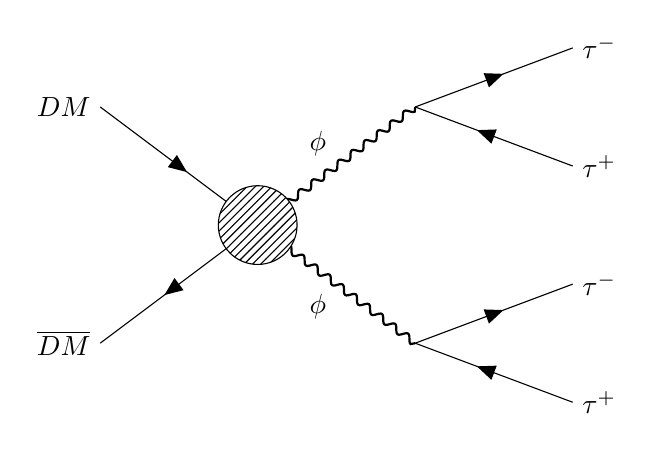
\begin{tikzpicture}
		\begin{feynman}
			% Define the vertices
			\vertex (c) at (0, 0); % Central point

			% Incoming Dark Matter (DM) particles
			\vertex (dm1) [label=left:\(DM\)] at (-2, 1.5);
			\vertex (dm2) [label=left:\(\overline{DM}\)] at (-2, -1.5);

			% Intermediate vertices for V decay
			\vertex (v1) at (2, 1.5);
			\vertex (v2) at (2, -1.5);

			% Outgoing Standard Model (SM) particles
			\vertex (sm1) [label=right:\(\tau ^-\)] at (4, 2.25);
			\vertex (sm2) [label=right:\(\tau ^+\)] at (4, 0.75);
			\vertex (sm3) [label=right:\(\tau ^-\)] at (4, -0.75);
			\vertex (sm4) [label=right:\(\tau ^+\)] at (4, -2.25);

			% Draw the diagram edges (particles and propagators)
			\diagram* {
			(dm1) -- [fermion] (c),
			(dm2) -- [anti fermion] (c),
			(c) -- [photon, thick, edge label=\(\phi \)] (v1),
			(c) -- [photon, thick, edge label'=\(\phi \)] (v2),
			(v1) -- [fermion] (sm1),
			(v1) -- [anti fermion] (sm2),
			(v2) -- [fermion] (sm3),
			(v2) -- [anti fermion] (sm4),
			};
	
			\vertex[blob, fill=white, draw=black, postaction={pattern=north east lines}, minimum size=1cm] at (c) {}; % Hatched central vertex
		\end{feynman}
	\end{tikzpicture}
	\caption{The Feynman diagram for the secluded dark matter model we are investigating. Two dark matter particles annihilate into two mediators \(\phi \) that later decay to \(4\tau \) leptons.}
	\label{fig:feynman}
\end{figure}

\section{The impact of Sommerfeld enhancement}
The annihilation cross-section of two dark matter particles into two mediators can be derived in quantum field theory and is independent of velocity. It can be expressed as
\begin{equation}
	\sigma v = \frac{\pi \alpha^2}{M_{DM}^2},
\end{equation}
% TODO: spiegare cosa è la dark matter relic abundance?
where \(\alpha\) is the strength of the interaction and \(M_{DM} \) is the mass of the dark matter particle. For non-self-conjugate dark matter, the value of the annihilation cross-section that gives the correct dark matter relic abundance for \(M_{DM} > 10 \mathrm{GeV} \) is \(\langle \sigma v \rangle _{relic}  = 4.4 \times 10^{-26} \mathrm{cm^{-3} s^{-1}}\). Without Sommerfeld enhancement, this enforces a linear relation between the strength of the interaction and the mass of the dark matter particles:
\begin{equation}
	\alpha(M_{DM} ) = M_{DM} \sqrt{\frac{\langle \sigma v \rangle _{relic}}{\pi}}
\end{equation}

If Sommerfeld enhancement is relevant at the time of freeze-out, the situation is different, because the cross-section must be corrected by multiplying by the Sommerfeld enhancement factor from Eq. \eqref{deriv:result}. The parameter \(\alpha \) must then satisfy the following equation:
\begin{equation}\label{eq:relic_Sommerfeld}
	\langle \sigma v \rangle _{relic} = \frac{2\pi \alpha ^3}{M_{DM} ^2} \frac{1 / v}{1- e^{-2\pi \frac{\alpha}{v}}},
\end{equation}
where \(v\) is the relative velocity between the two dark matter particles, which at freeze-out satisfies
\begin{equation}
	\left \langle \frac{1}{v} \right \rangle \simeq 4
\end{equation}
More precisely, one should compute a thermal average of the Sommerfeld enhancement factor and use that in Eq. \eqref{eq:relic_Sommerfeld}, but at these velocities the difference between an averaged enhancement factor and the same factor calculated at \(v= \langle v \rangle \) is almost non-existent. Equation \eqref{eq:relic_Sommerfeld} does not have an analytic solution and must therefore be solved with numerical tools. Fig. \ref{fig:alpha} compares \(\alpha (M_{DM} )\) in the two cases and shows that the difference becomes noticeable for masses around \(1 \mathrm{TeV} \).

\begin{figure}[htbp]
	\centering
	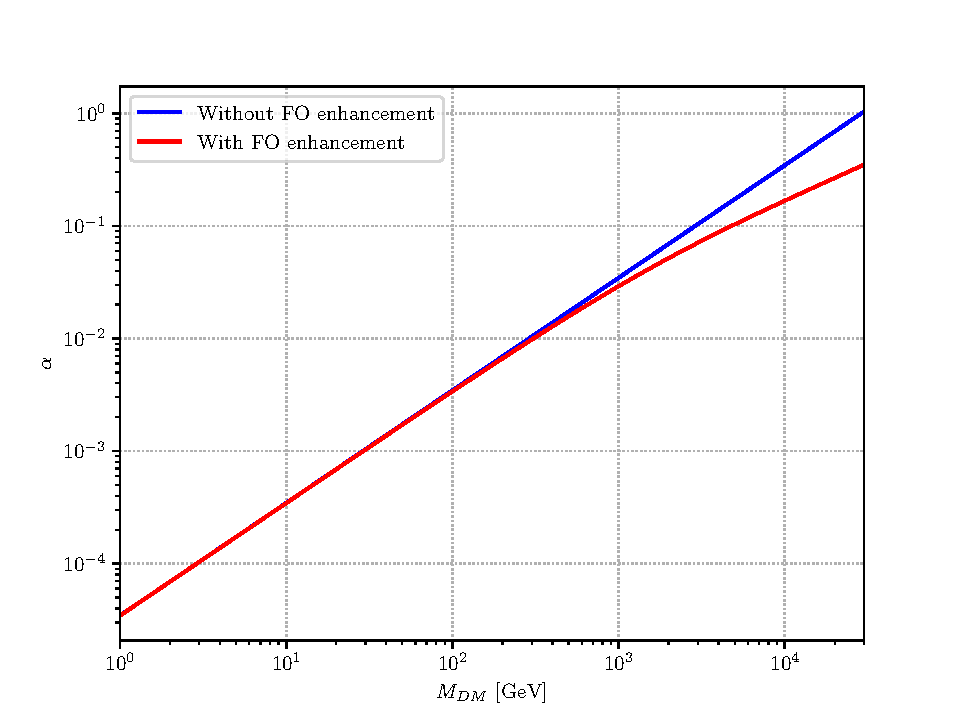
\includegraphics[width=\textwidth]{alpha.pdf}
	\caption{Comparison between the \(\alpha (M_{DM} )\) relations with and without Sommerfeld enhancement at freeze-out, in red and blue respectively. \(\langle 1 / v \rangle \simeq 4 \) at freeze-out.}
	\label{fig:alpha}
\end{figure}

We can now use the corrected \(\alpha (M_{DM} )\) dependence to plot the Sommerfeld enhancement factor (Fig. \ref{fig:enhancement_factor}) against the relative velocity in units of \(c\) and confirm that it has indeed a huge impact on the cross-section (\(2-3\) orders of magnitude) at low velocities like those found in dSphs.

\begin{figure}[htbp]
	\centering
	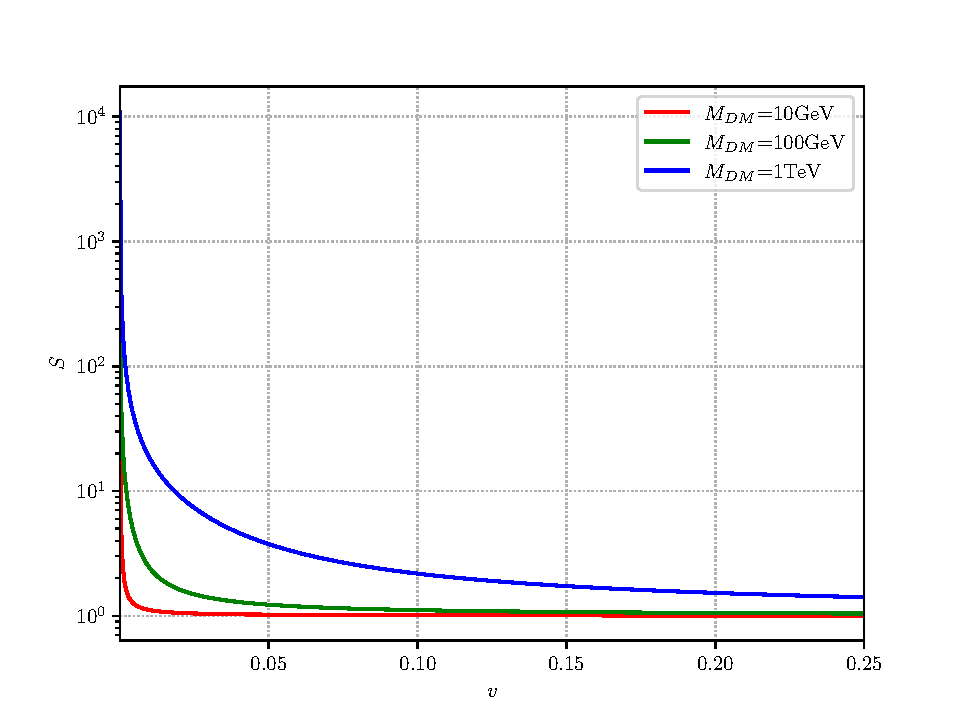
\includegraphics[width=\textwidth]{enhancement_factor.pdf}
	\caption{The Sommerfeld enhancement factor for three different values of \(M_{DM} \). The graph ranges from the typical velocities in dSphs (\(\sim 10 \mathrm{km / s} \)) to the characteristic velocity at freeze-out (\(\langle 1 / v \rangle \simeq 4\)).}
	\label{fig:enhancement_factor}
\end{figure}

The predicted cross-section with the corrected \(\alpha (M_{DM} )\) is
\begin{equation}\label{eq:sigma_enhanced}
	\langle \sigma v \rangle (M_{DM} )= \frac{\pi \alpha (M_{DM} )^2}{M_{DM} ^2} \left \langle S \right \rangle(M_{DM} ),
\end{equation}
where the angle brackets indicate a thermal average over the Maxwell-Boltzmann distribution for the relative velocity. Here, averaging over the distribution is more important compared to the case at freeze-out and \(\langle S \rangle \neq S|_{v= \langle v \rangle }\). One can show that the relative velocity dispersion \(\beta_{rel} \) is related to the single-particle velocity dispersion \(\beta \) by \(\beta _{rel} = \sqrt{2} \beta \) (See Appendix \ref{appendix:1d}), therefore the relative velocity PDF is
\begin{equation}
	P(v ) = \left( \frac{1}{4\pi } \right)^\frac{1}{2} \frac{v ^2}{\beta ^3} \exp \left( -\frac{v ^2}{4 \beta ^2} \right),
\end{equation}
where I am using \(\beta = 10 \mathrm{km / s} \) for a typical dSph \cite{Walker_2013, Arkani_2009}.
The averaged Sommerfeld enhancement factor, which I computed numerically, is therefore
\begin{equation}
	\langle S \rangle (M_{DM} ) = \int\limits_0^{+ \infty } P(v ) S(M_{DM}, v ) \mathrm{d} v
\end{equation}


\section{Results}\label{sec:results}
In the simple case of no Sommerfeld enhancement and therefore of a linear \(\alpha (M_{DM} )\), the predicted cross-section is
\begin{equation}
	\langle \sigma v \rangle = \langle \sigma v \rangle _{relic}
\end{equation}
for any value of \(M_{DM} \). Since the Fermi-LAT limits are upper bounds on the cross-section, we want the predicted cross-section to be lower than the limits and this constrains the dark matter mass to be
\begin{equation}\label{eq:result_simple}
	M_{DM} \gtrsim 82 \mathrm{GeV}, 
\end{equation}
which is where the horizontal line of \(\langle \sigma v \rangle _{relic} \) and the weakened Fermi-LAT limits meet in Fig. \ref{fig:comparison}.

To perform the same analysis for the Sommerfeld-enhanced case, we need to slightly extend the experimental limits further than \(10 \mathrm{TeV} \). This can be done by fitting the weakened Fermi-LAT data to a function that looks like a parabola in a double-log plot:
\begin{equation}
	f(M_{DM} ;K,M_0,a,b) = K \left( \frac{M_{DM} }{M_0} \right) ^ {-a-b \ln (M_{DM} / M_0)},
\end{equation}
where \(K, M_0, a,\) and \(b\) are parameters that are determined using non-linear least squares fitting. The fitted function is shown in Fig. \ref{fig:comparison} as a continuous black line. It can be seen that it fits very well with the experimental data above \(1\mathrm{TeV} \). The enhanced cross-section from Eq. \ref{eq:sigma_enhanced} is shown as a continuous red line. Numerically, we can solve the equation
\begin{equation}
	\langle \sigma v \rangle (M_{DM} ) = f(M_{DM} ; K,M_0,a,b) 
\end{equation}
to find where limits and theoretical prediction meet. Following the same reasoning as before, we find that
\begin{equation}\label{eq:result_enhanced}
	M_{DM} \gtrsim 12 \mathrm{TeV}
\end{equation}
in the case with Sommerfeld enhancement. Figure \ref{fig:comparison} summarizes these findings and clearly shows where the constraints come from. Comparing between Eq. \ref{eq:result_simple} and Eq. \ref{eq:result_enhanced} shows that the presence of Sommerfeld enhancement can impact by orders of magnitude the constraints we put on the dark matter mass.

\begin{figure}[htbp]
	\centering
	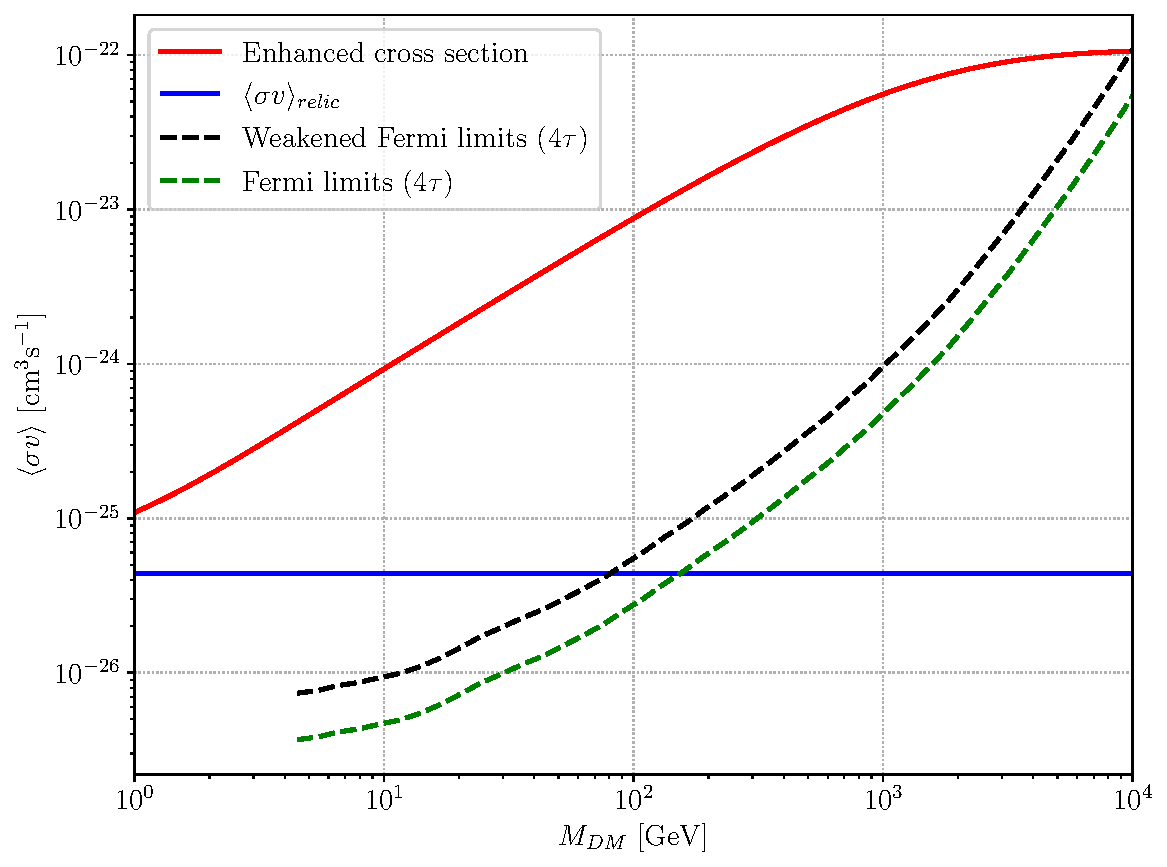
\includegraphics[width=\textwidth]{comparison.pdf}
	\caption{Comparison between theoretical prediction and experimental limits set by Fermi-LAT data.}
	\label{fig:comparison}
\end{figure}

\section{Checking the Coulomb approximation}

We must now check whether using the Coulomb approximation was appropriate in this case. The Coulomb approximation is valid if
\begin{equation}
	\frac{M_{DM} v}{2 m_{\phi } } \geq 1,
\end{equation}
As mentioned in Eq. \eqref{eq:mediator_mass}, \(m_{\phi } > 2 m_{\tau } \), and we have just found \(M_{DM} \gtrsim 12 \mathrm{TeV} \) in Eq. \eqref{eq:result_enhanced}. For the relative velocity \(v\), I am using its average value \(\langle v \rangle = 4 \beta /\sqrt{\pi } \) where \(\beta = 10 \mathrm{km / s} \) as before. Calculating this ratio with the minimum allowed masses yields \(\sim 0.13\), meaning that the Coulomb approximation is actually not a good approximation in this case. Still, it gives us a good idea of the great effect that the Sommerfeld enhancement can have on constraints that we put on dark matter mass.

Since the Coulomb approximation is not valid in this case, one should resort back to a Yukawa potential that does account for the mediator mass. In this case, the Schrödinger equation does not have an analytic solution and must be solved numerically. Alternatively, the Yukawa potential can be approximated by the Hulthen potential, which gives an equation that does have an analytic solution. The main qualitative difference in this case is that the Sommerfeld effect saturates at low velocities: the supposed dark force has a finite range, and this limits how big the enhancement can get. This will change the precise constraints on the mass, but the Sommerfeld enhancement will still be around the same order of magnitude \cite{Arkani_2009}.

\begin{appendices}
\chapter{Reduction to one-dimensional problem}\label{appendix:1d}
\end{appendices}

\chapter*{Acknowledgments}
\addcontentsline{toc}{chapter}{Acknowledgments}

\printbibliography[heading=bibintoc]
\end{document}
